%%%%\input{images/winlength}
%

\begin{figure}[!h]
\begin{center}{c}
 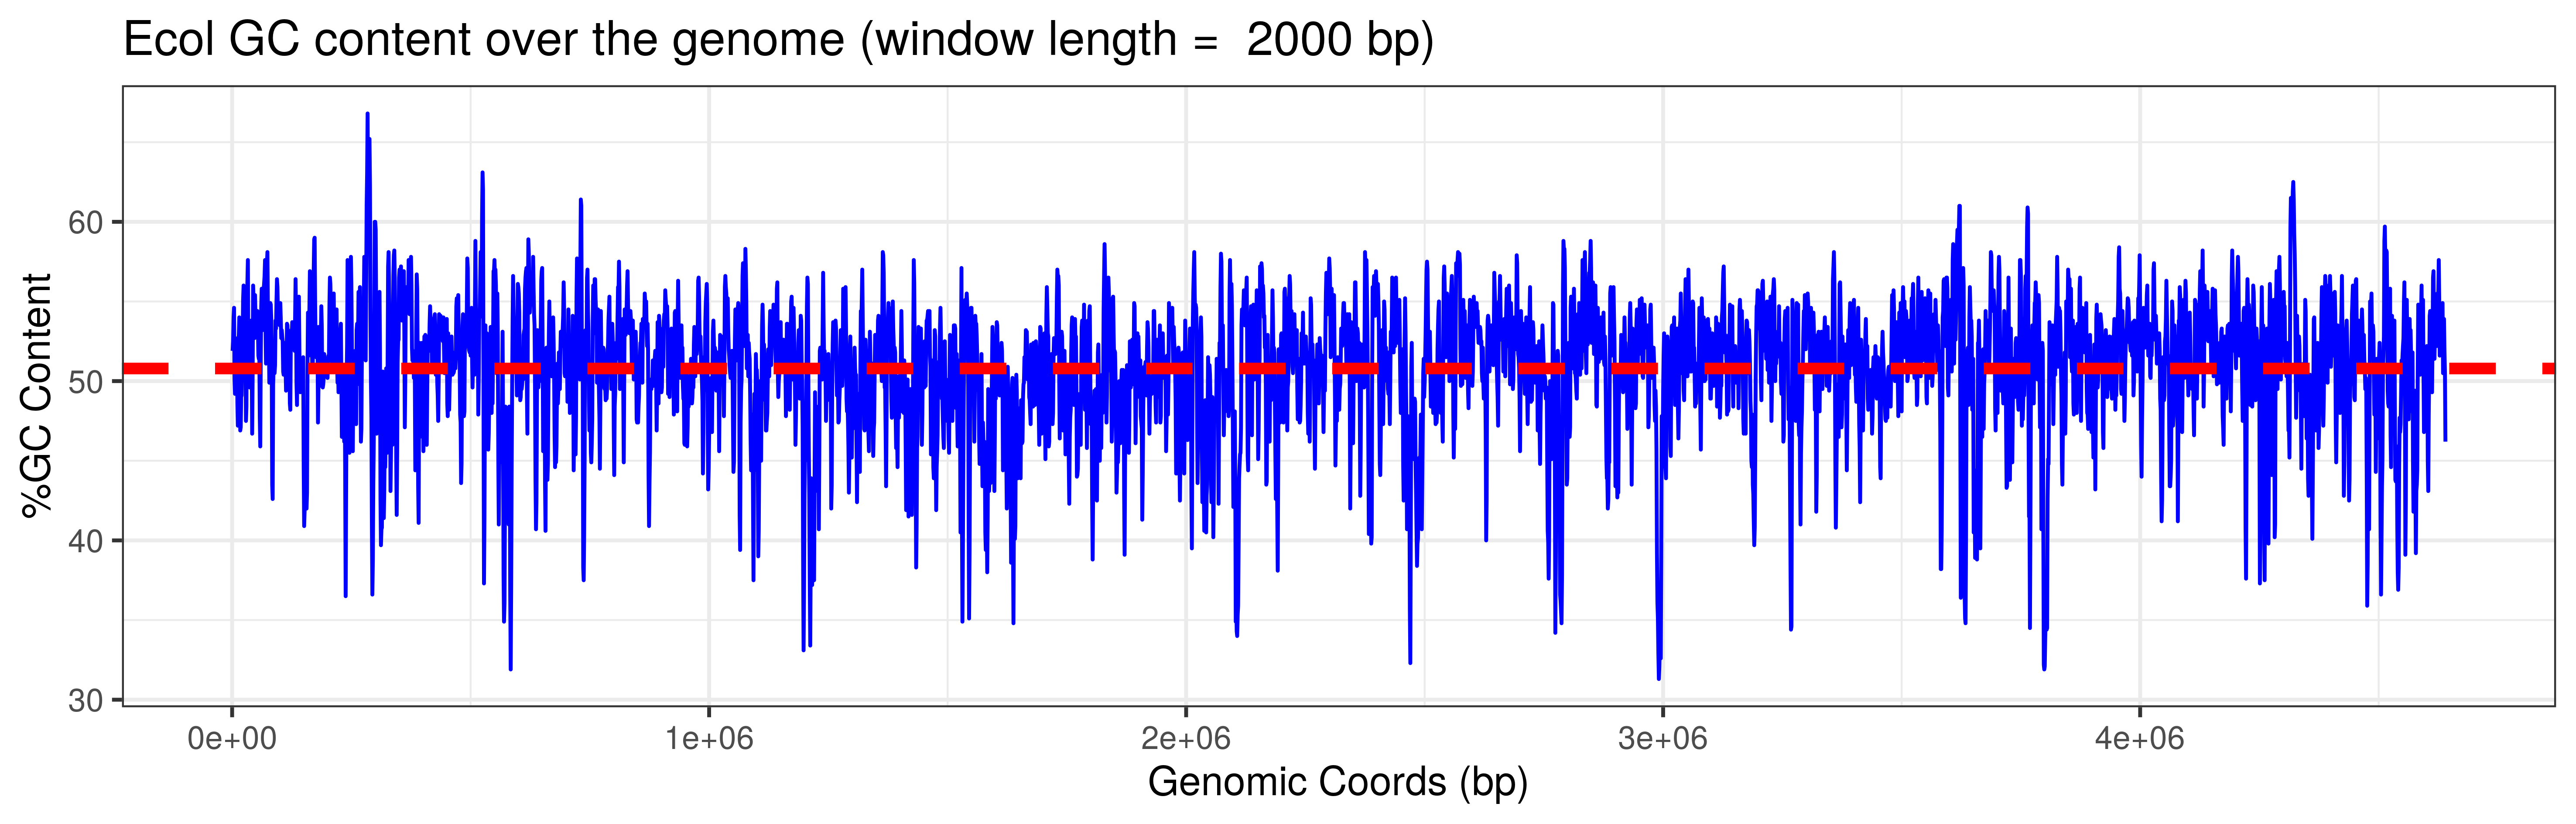
\includegraphics[width=0.5\linewidth]{{images/Ecol_genomegcanalysis_wlen2000}.png}\\
 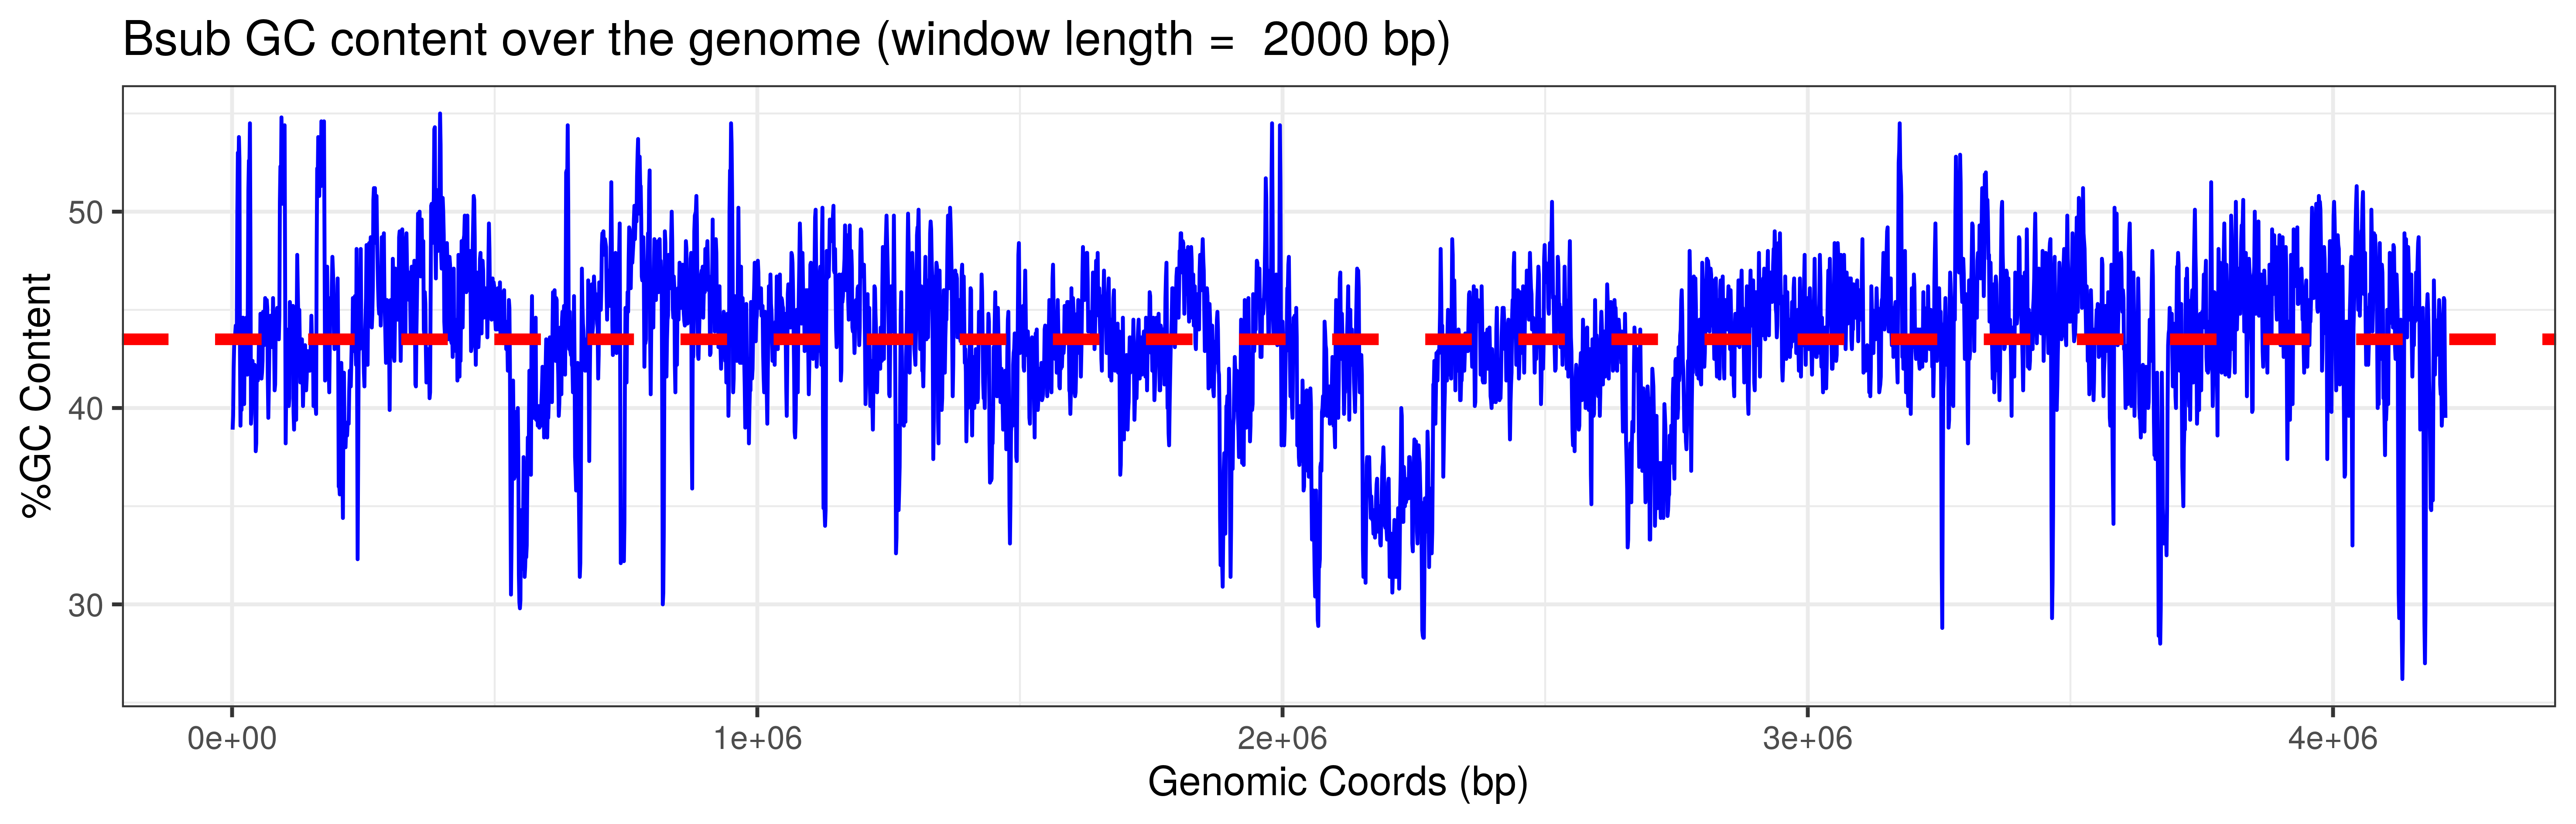
\includegraphics[width=0.5\linewidth]{{images/Bsub_genomegcanalysis_wlen2000}.png}\\
 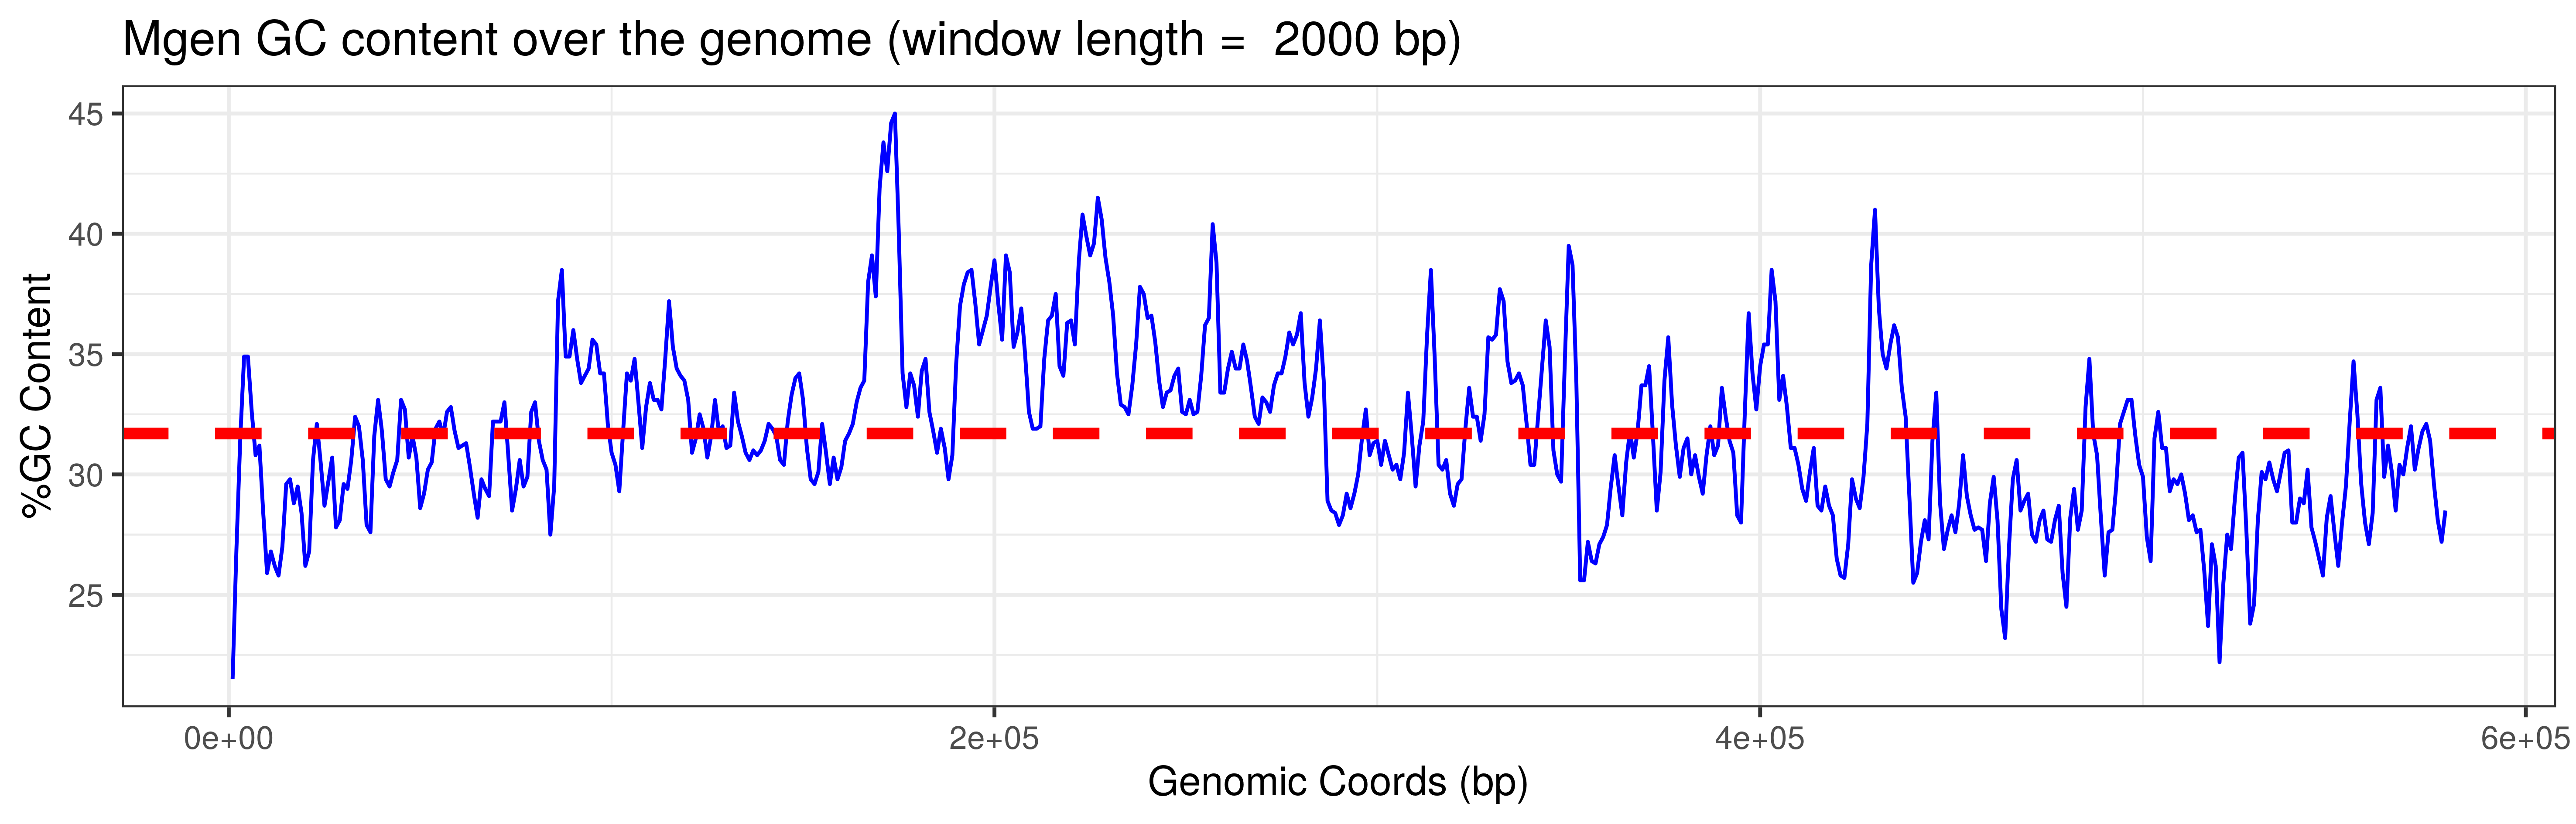
\includegraphics[width=0.5\linewidth]{{images/Mgen_genomegcanalysis_wlen2000}.png}\\
 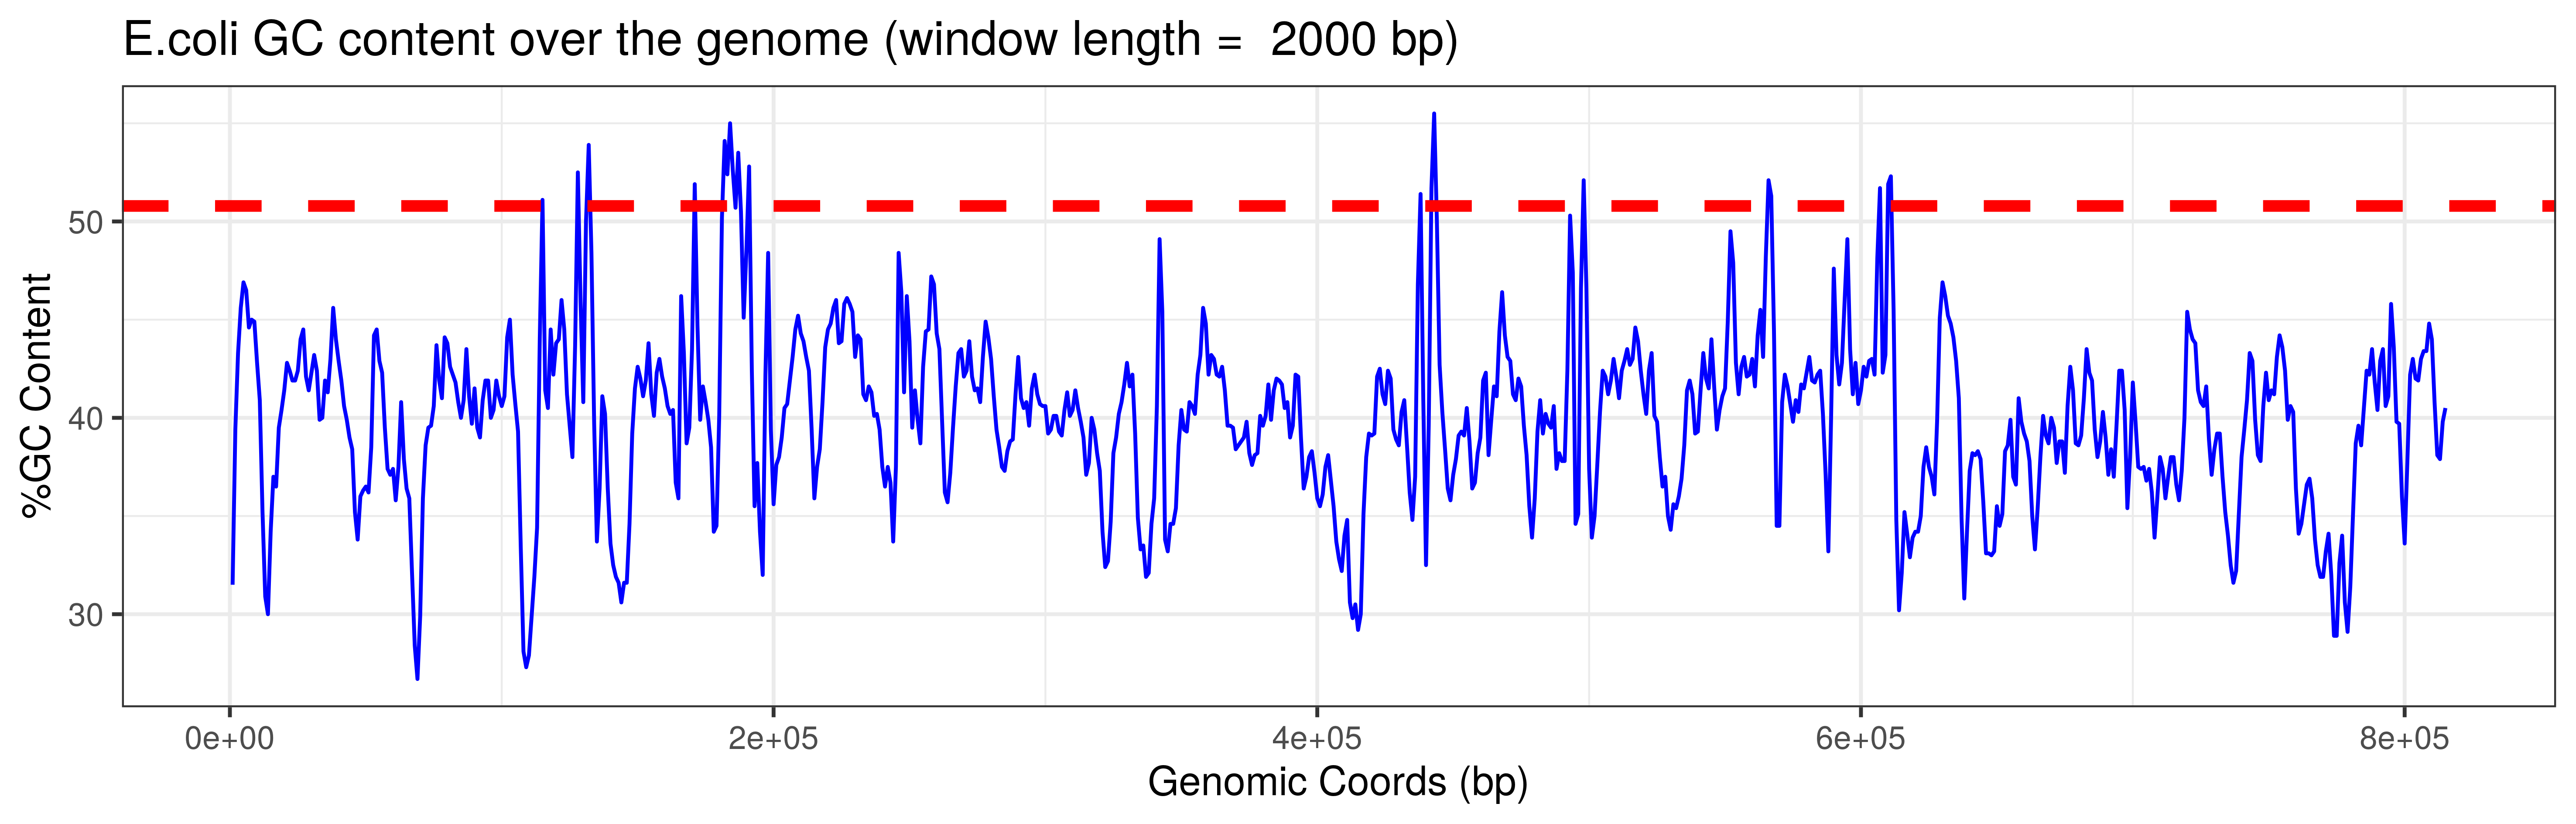
\includegraphics[width=0.5\linewidth]{{images/Mpne_genomegcanalysis_wlen2000}.png}\\
\end{center}

\caption[\cele\ Windows analysis for different genomes with windows size of 2000(bp).]{%
  \label{fig:winlength}\textbf{\cele\ Windows size analysis.}
}%
\end{figure}

%

\begin{figure}[!h]
\begin{center}{c}
 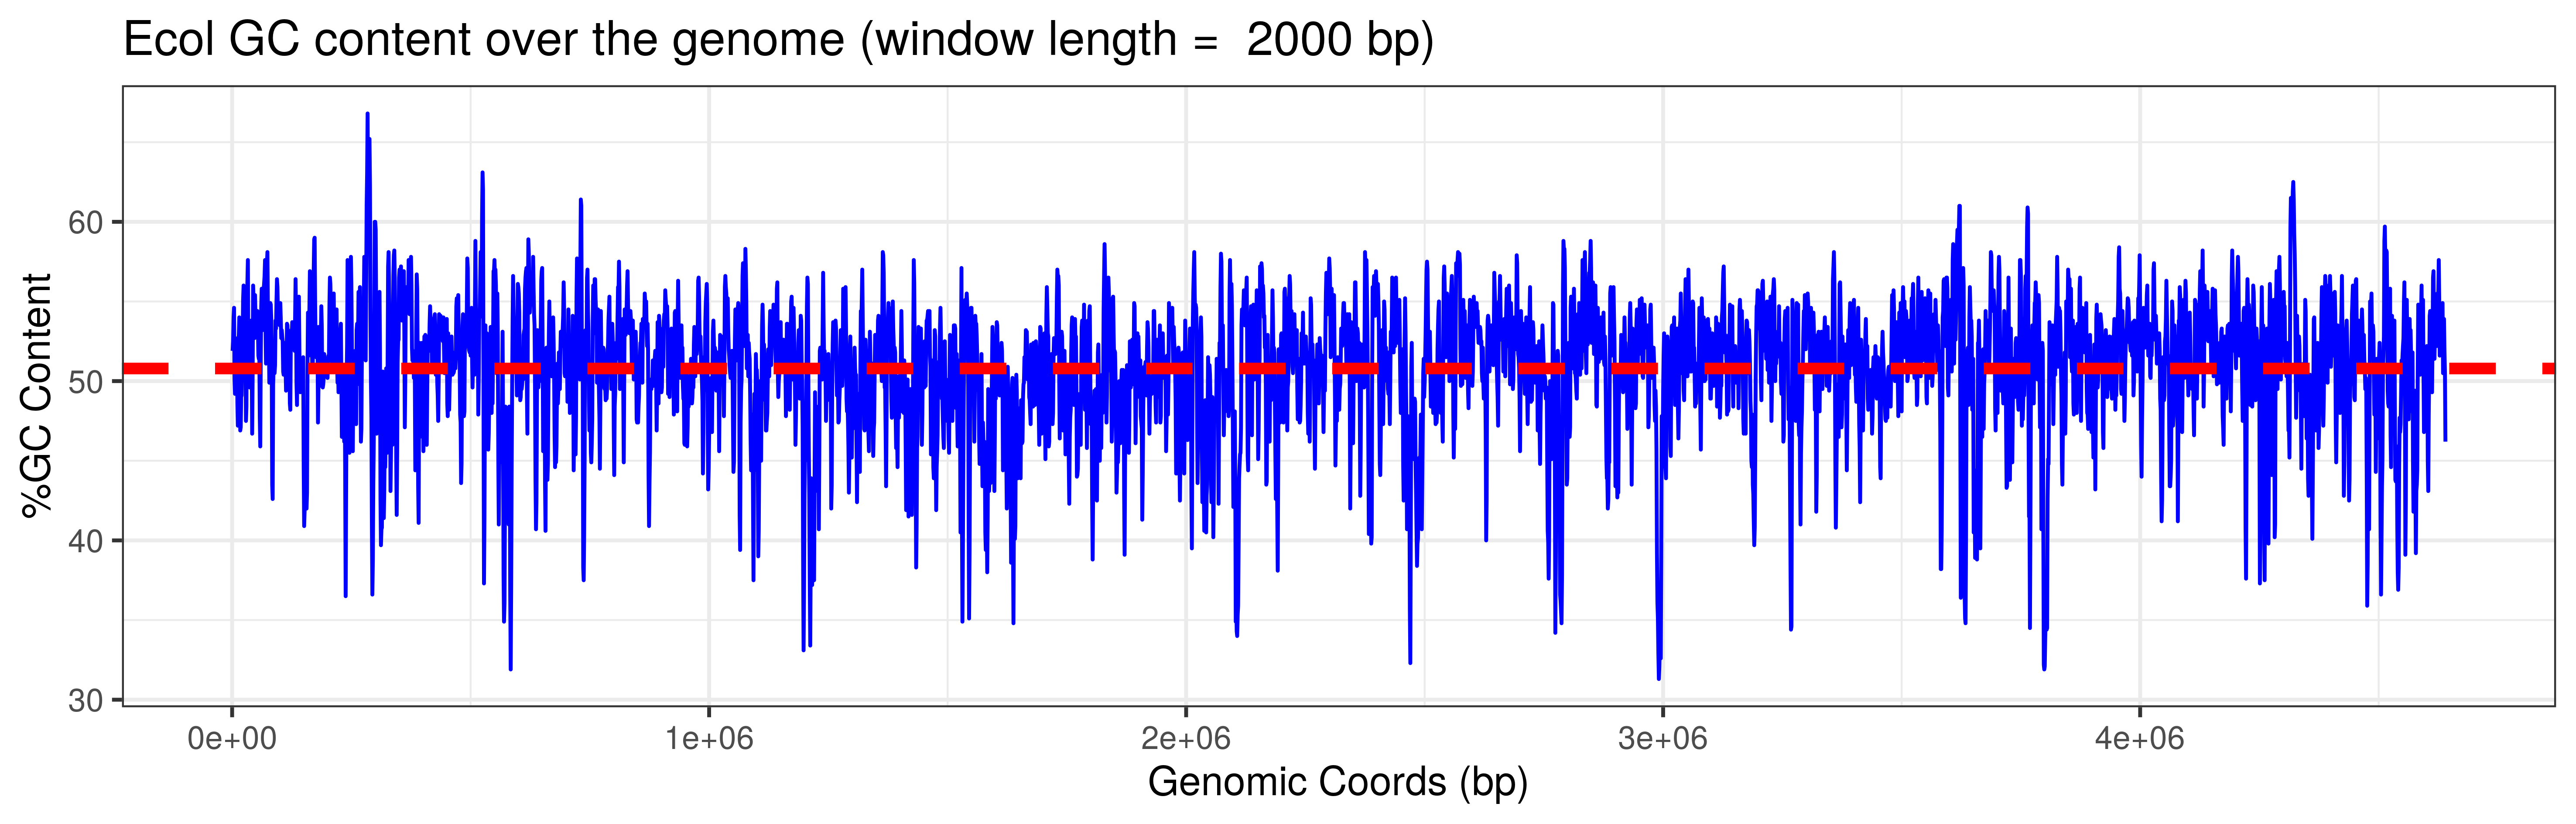
\includegraphics[width=0.5\linewidth]{{images/Ecol_genomegcanalysis_wlen2000}.png}\\
 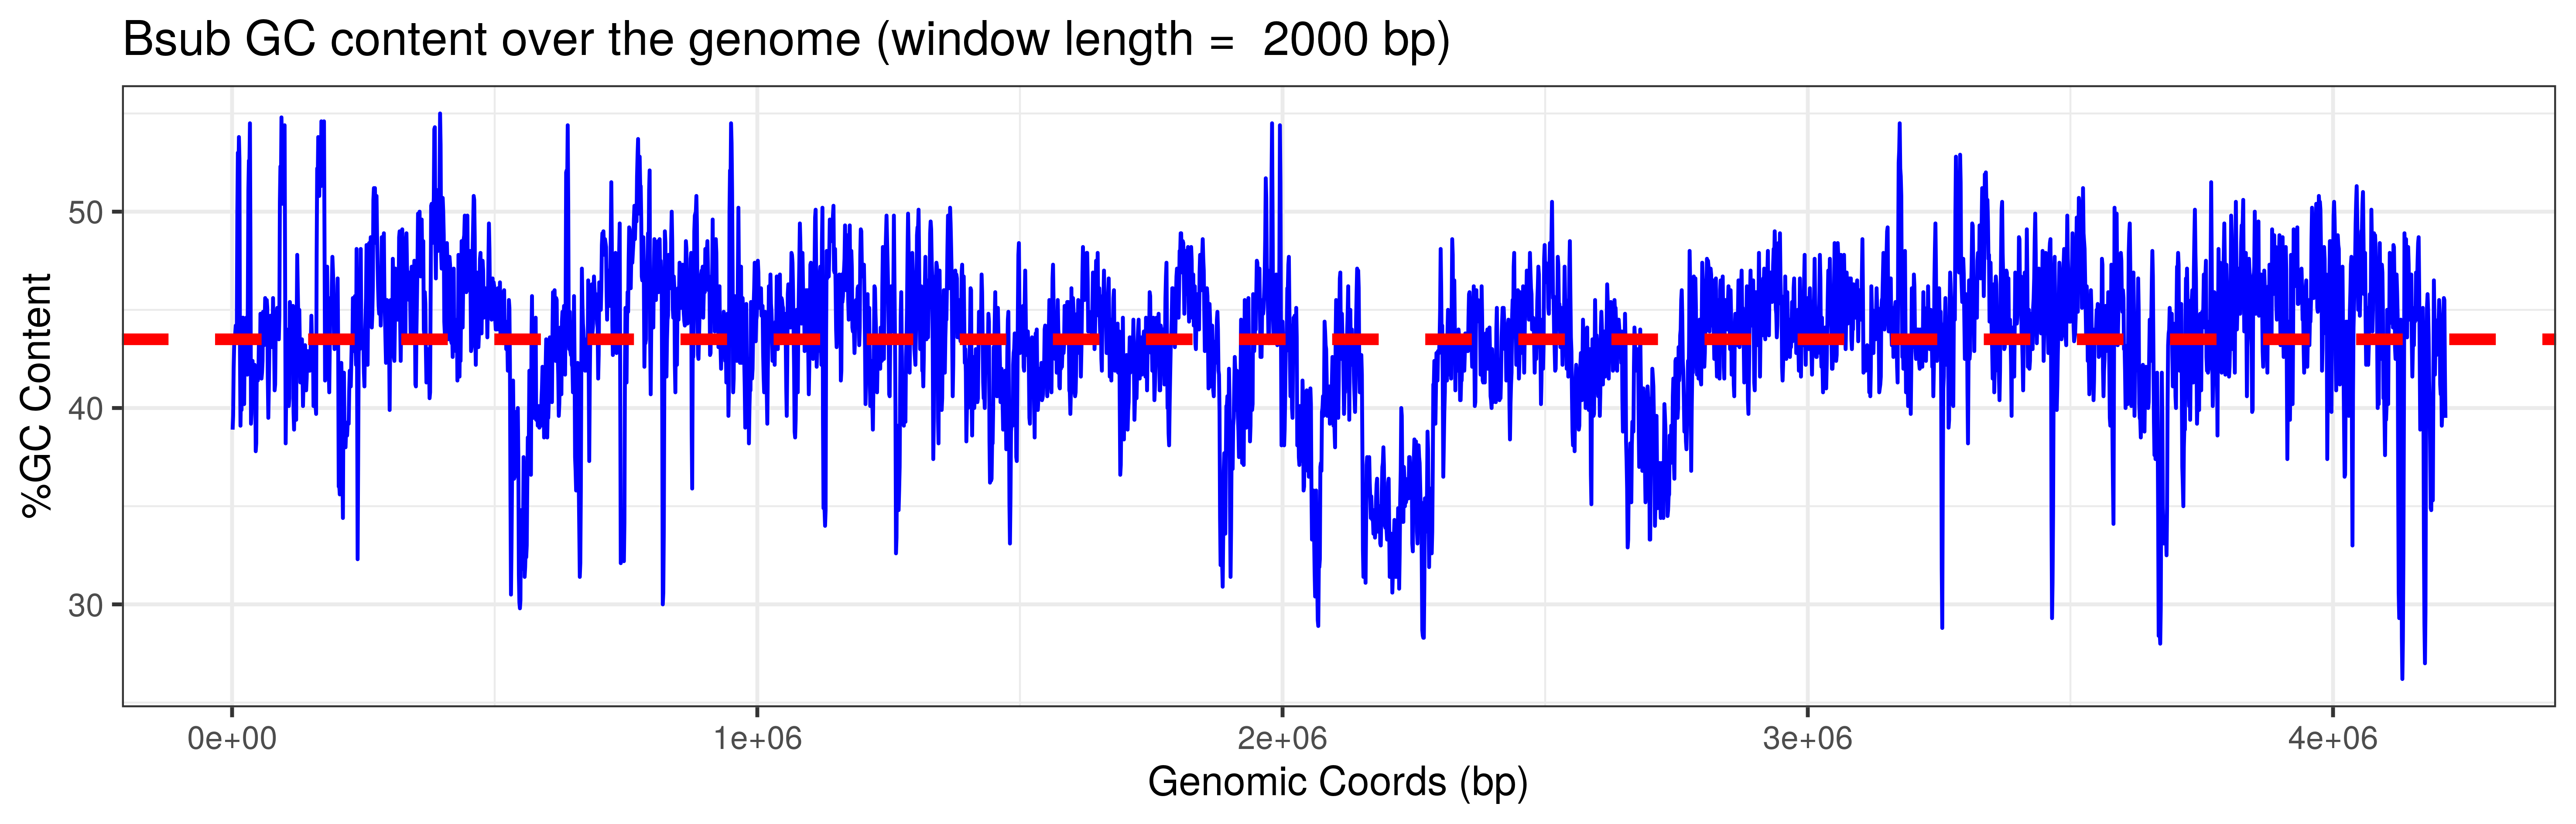
\includegraphics[width=0.5\linewidth]{{images/Bsub_genomegcanalysis_wlen2000}.png}\\
 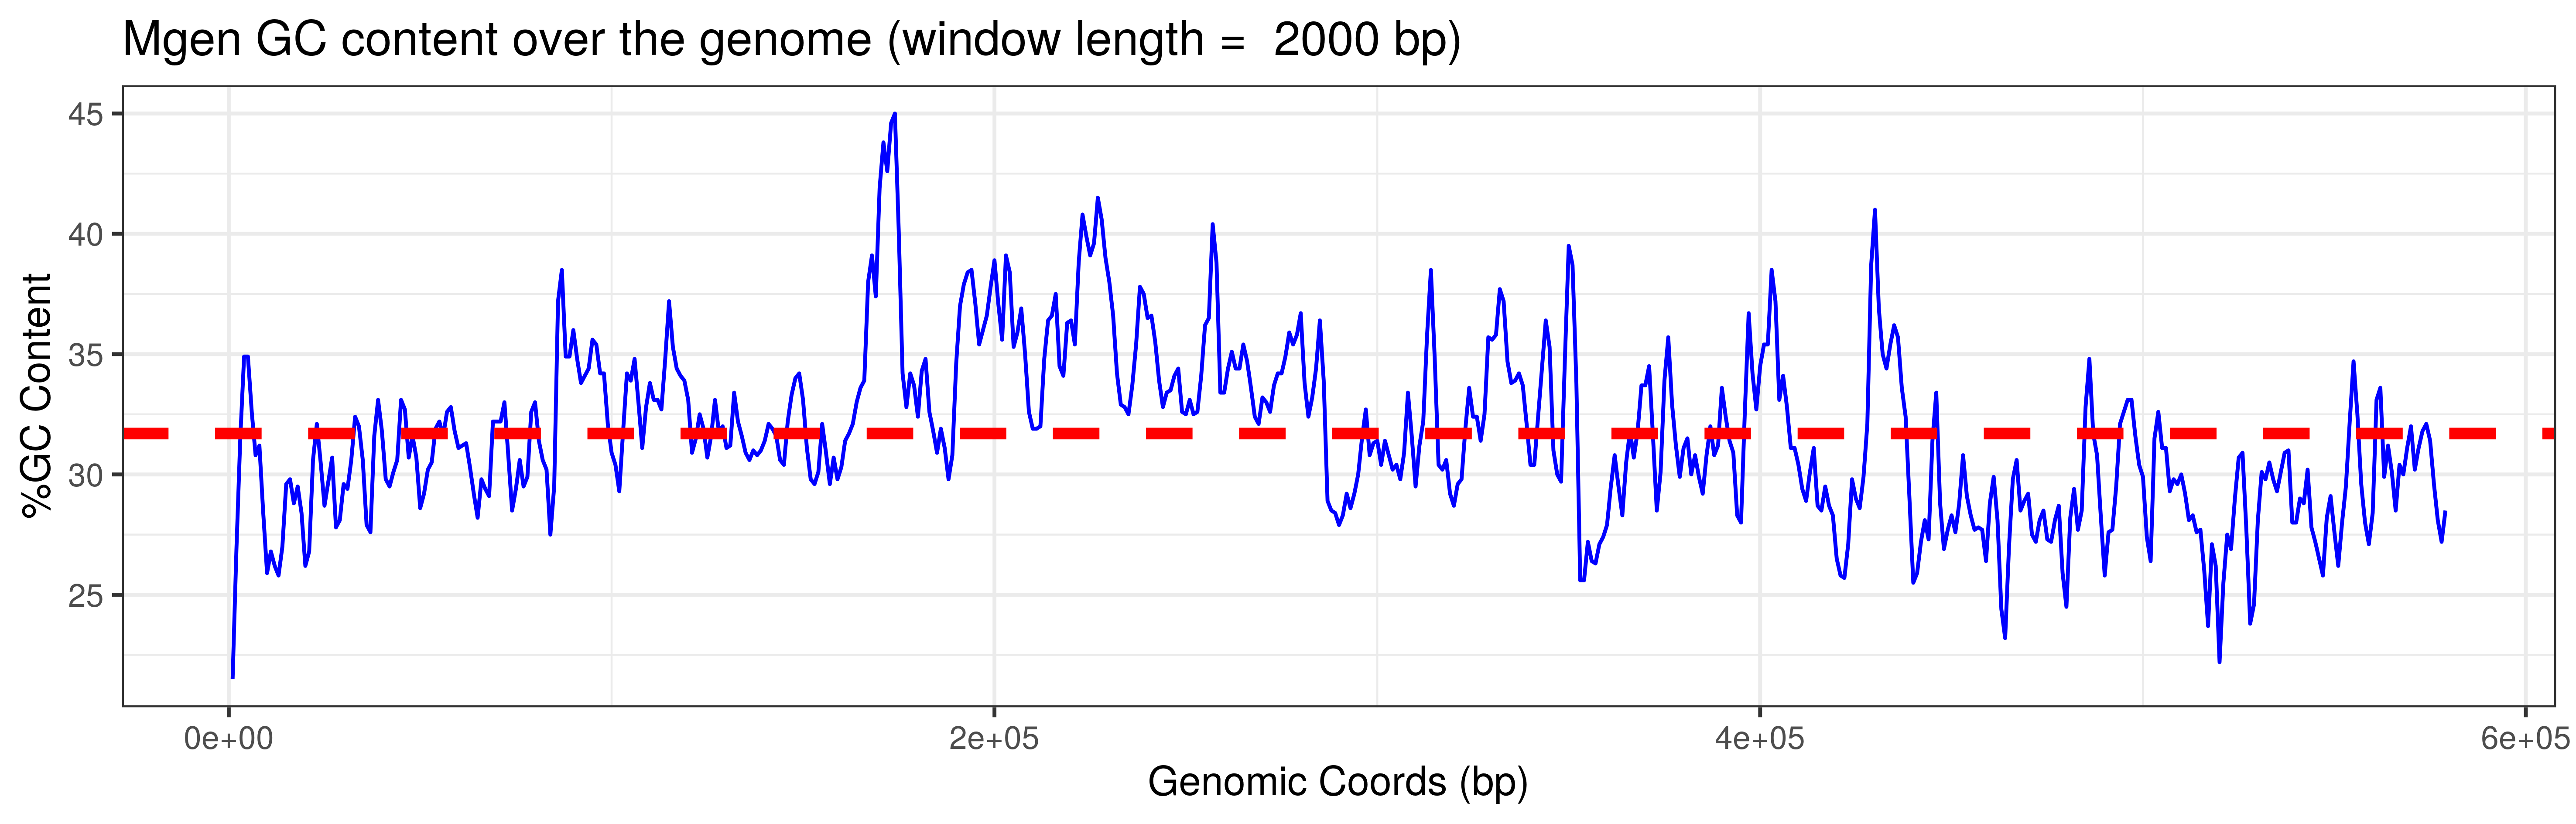
\includegraphics[width=0.5\linewidth]{{images/Mgen_genomegcanalysis_wlen2000}.png}\\
 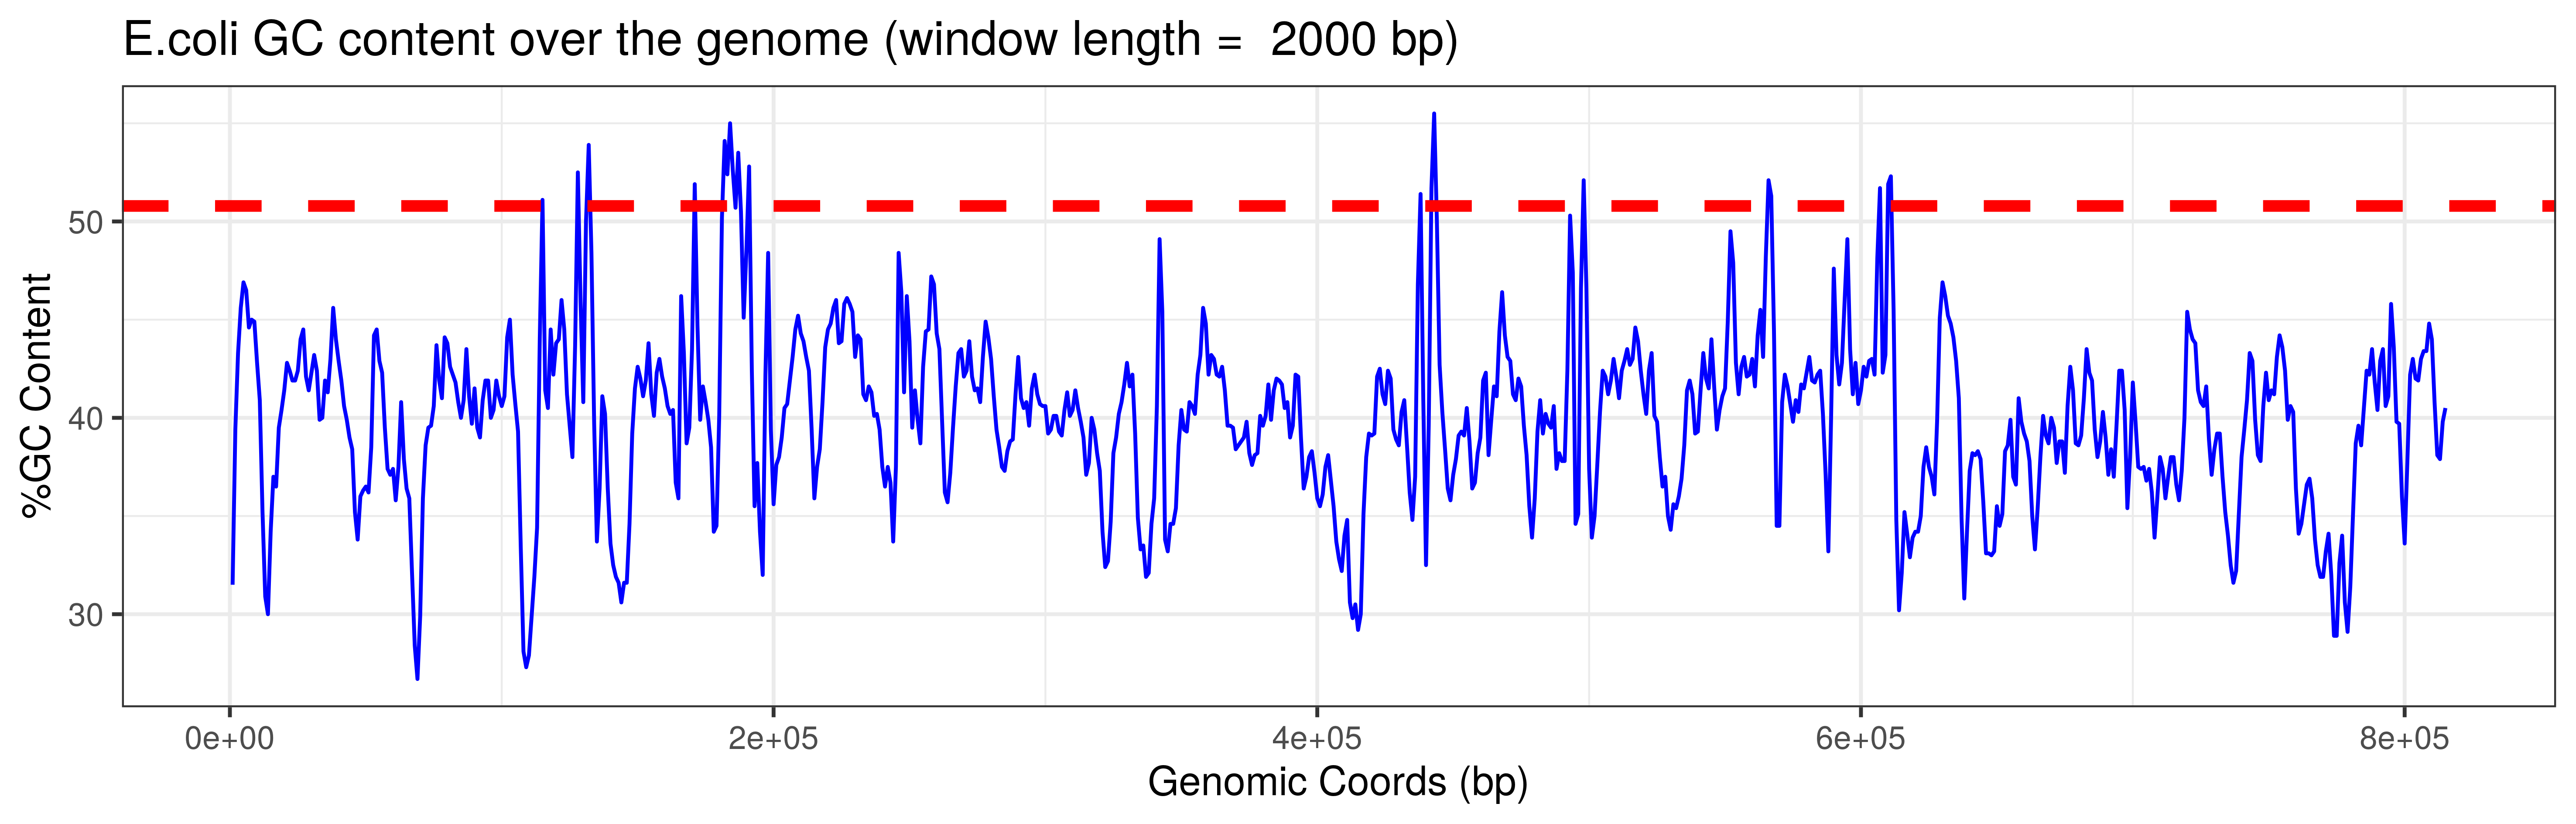
\includegraphics[width=0.5\linewidth]{{images/Mpne_genomegcanalysis_wlen2000}.png}\\
\end{center}

\caption[\cele\ Windows analysis for different genomes with windows size of 2000(bp).]{%
  \label{fig:winlength}\textbf{\cele\ Windows size analysis.}
}%
\end{figure}

%

\begin{figure}[!h]
\begin{center}{c}
 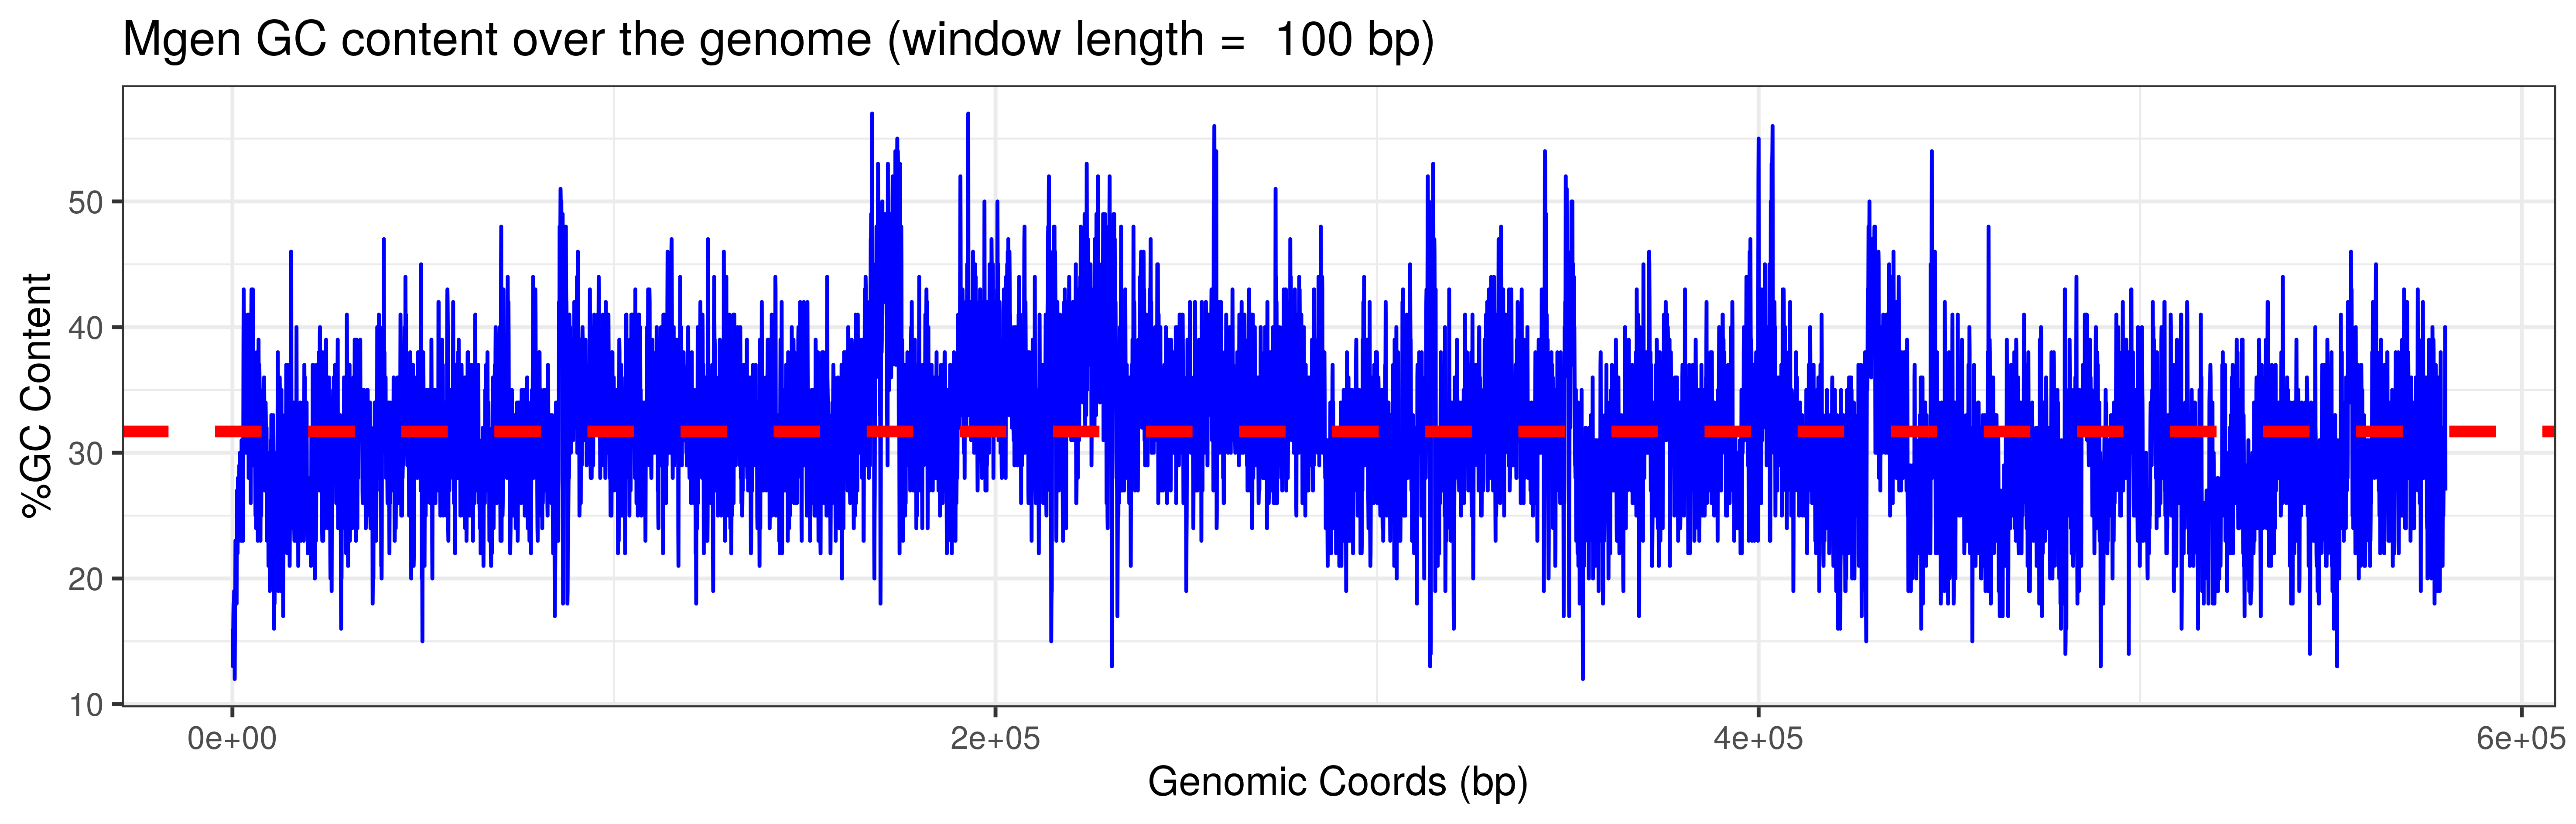
\includegraphics[width=0.5\linewidth]{{images/Mgen_genomegcanalysis_wlen100}.png}\\
 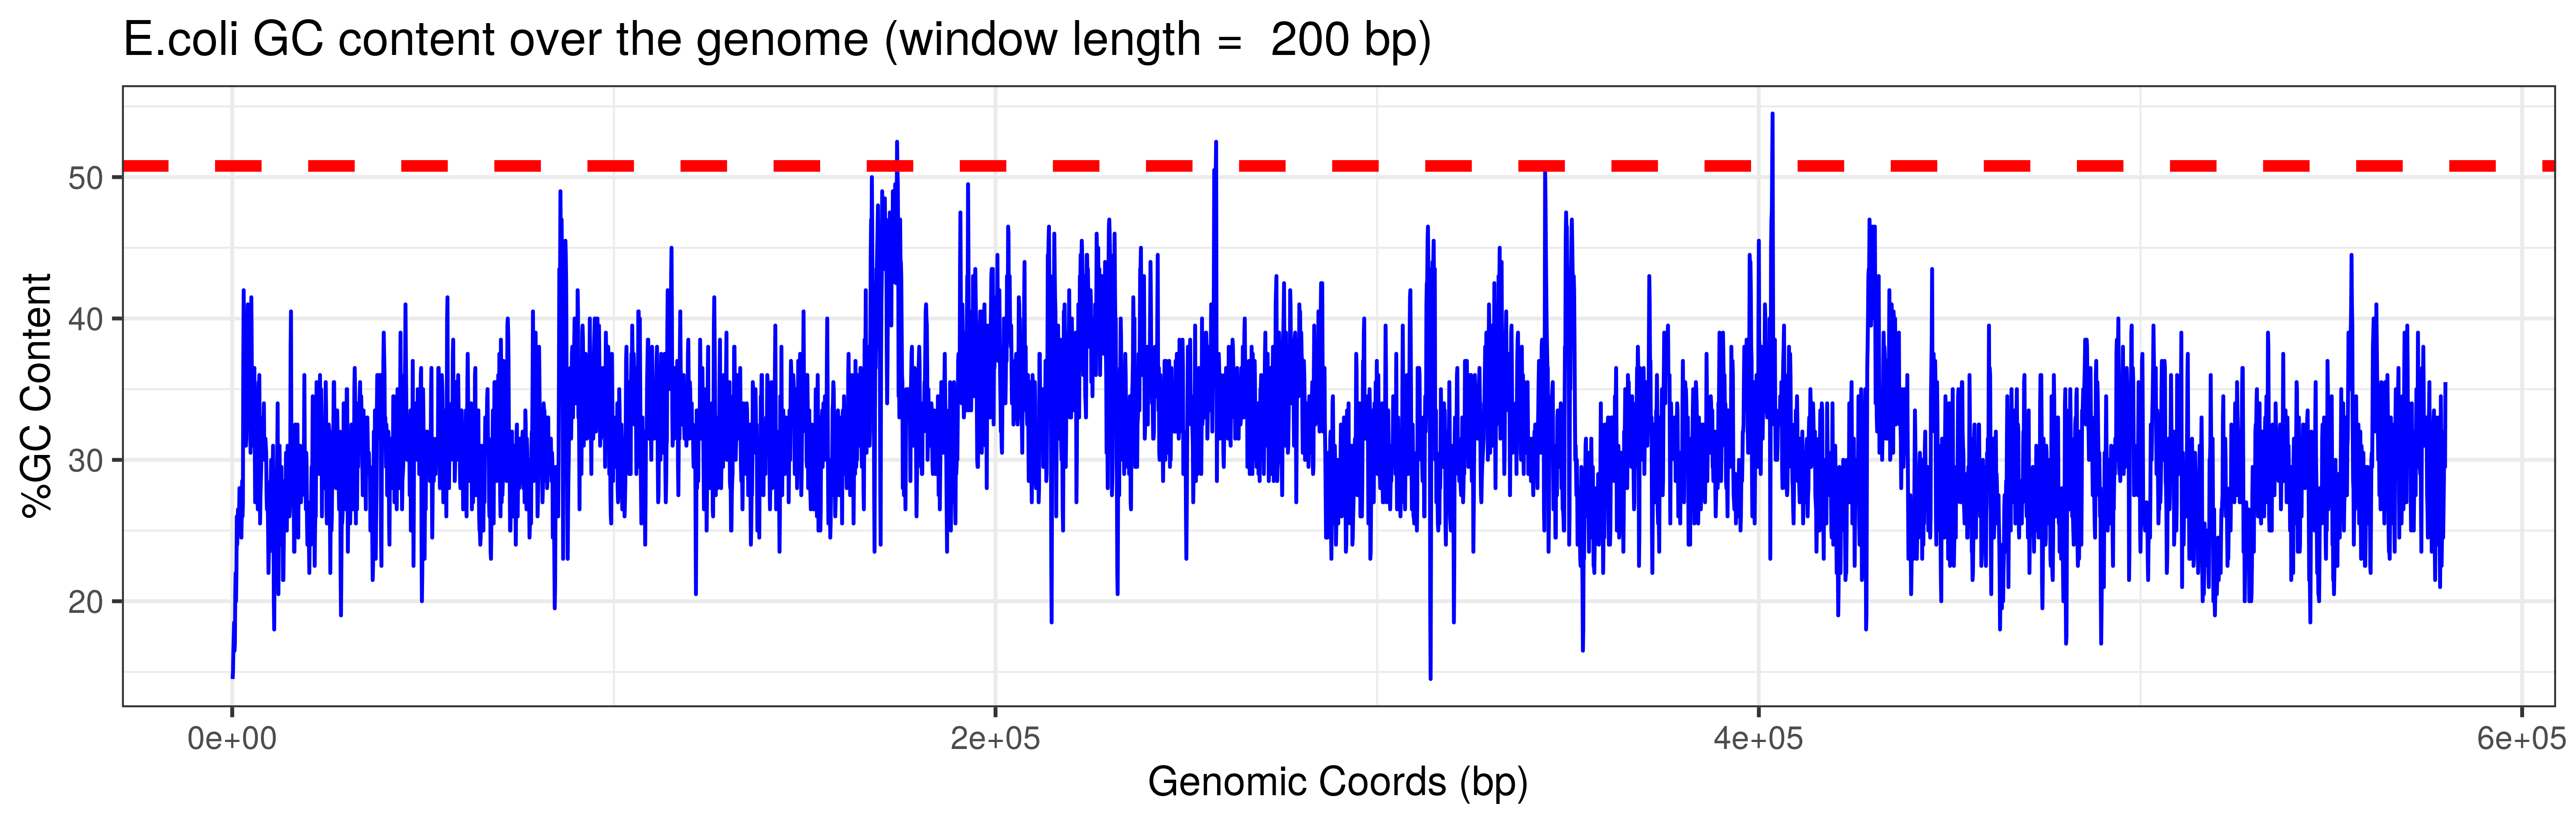
\includegraphics[width=0.5\linewidth]{{images/Mgen_genomegcanalysis_wlen200}.png}\\
 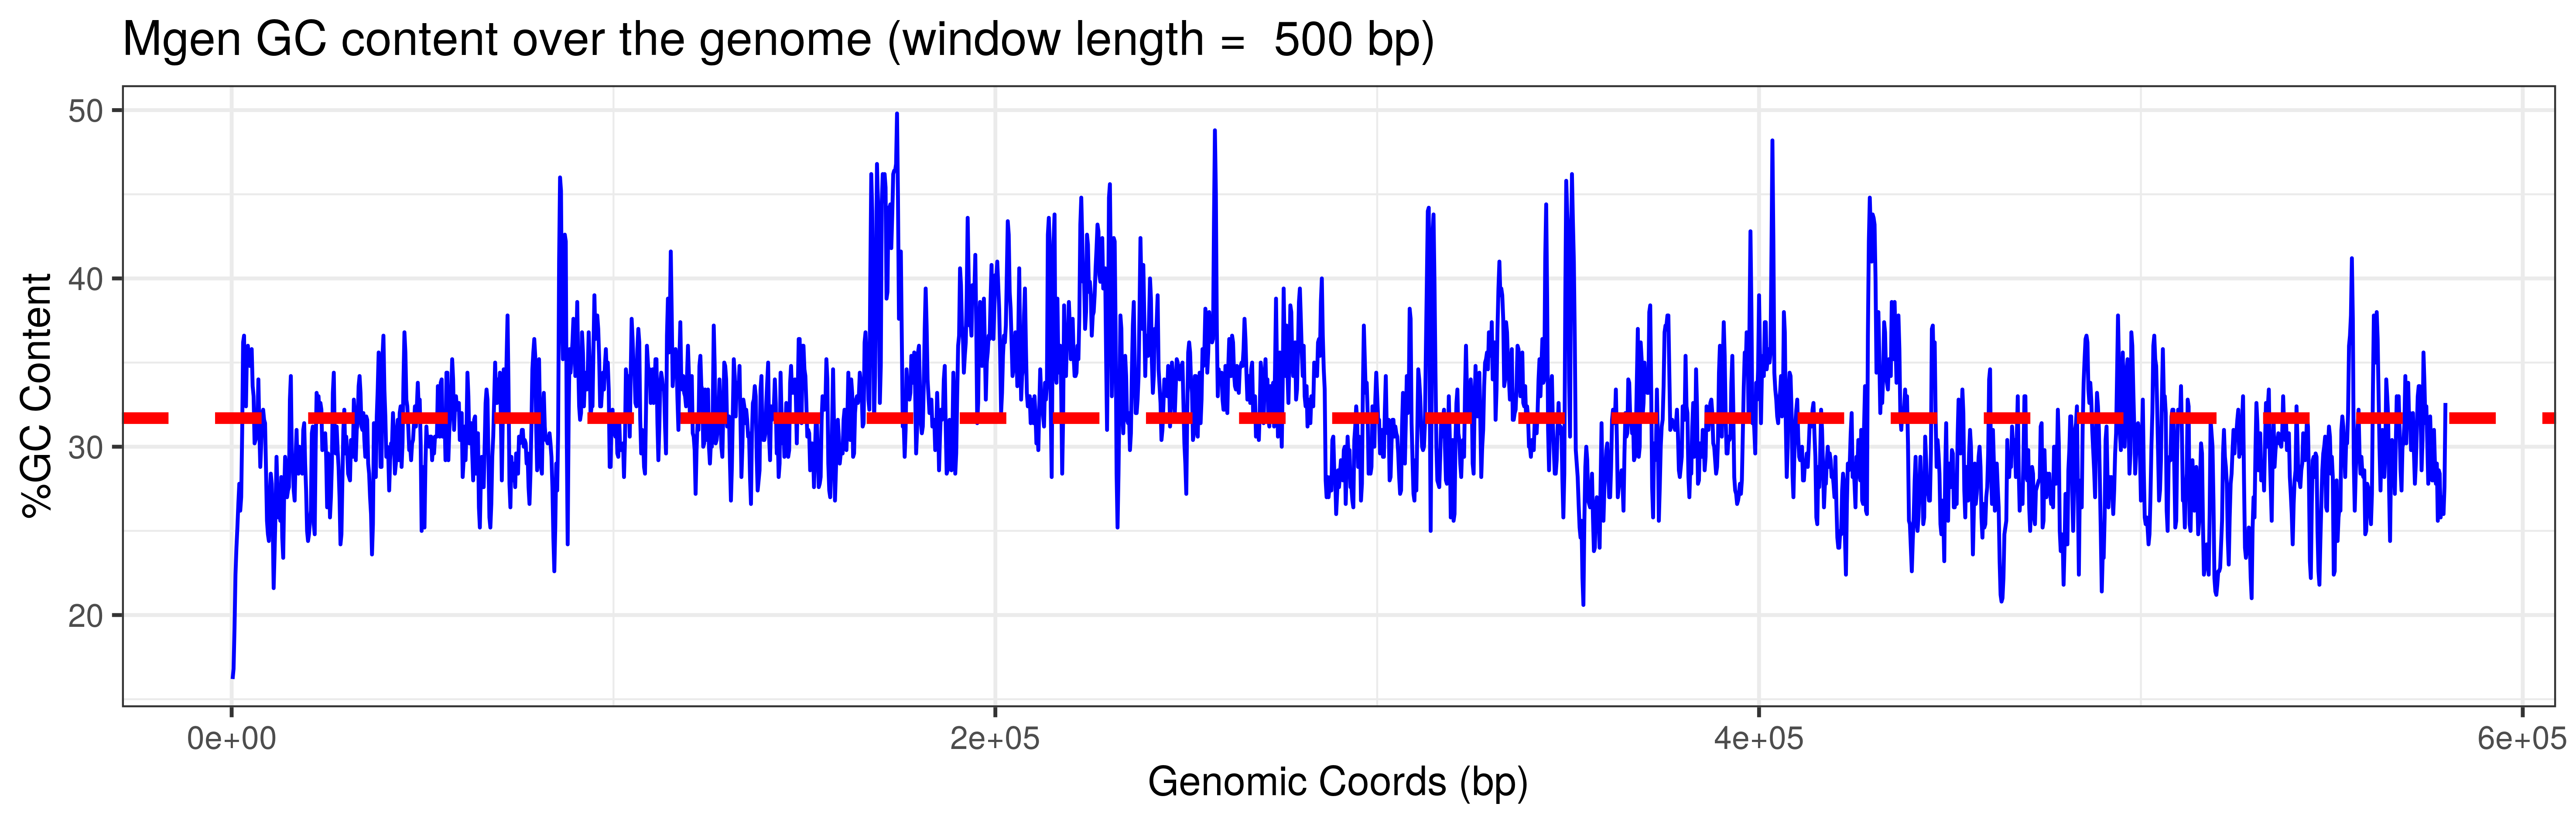
\includegraphics[width=0.5\linewidth]{{images/Mgen_genomegcanalysis_wlen500}.png}\\
 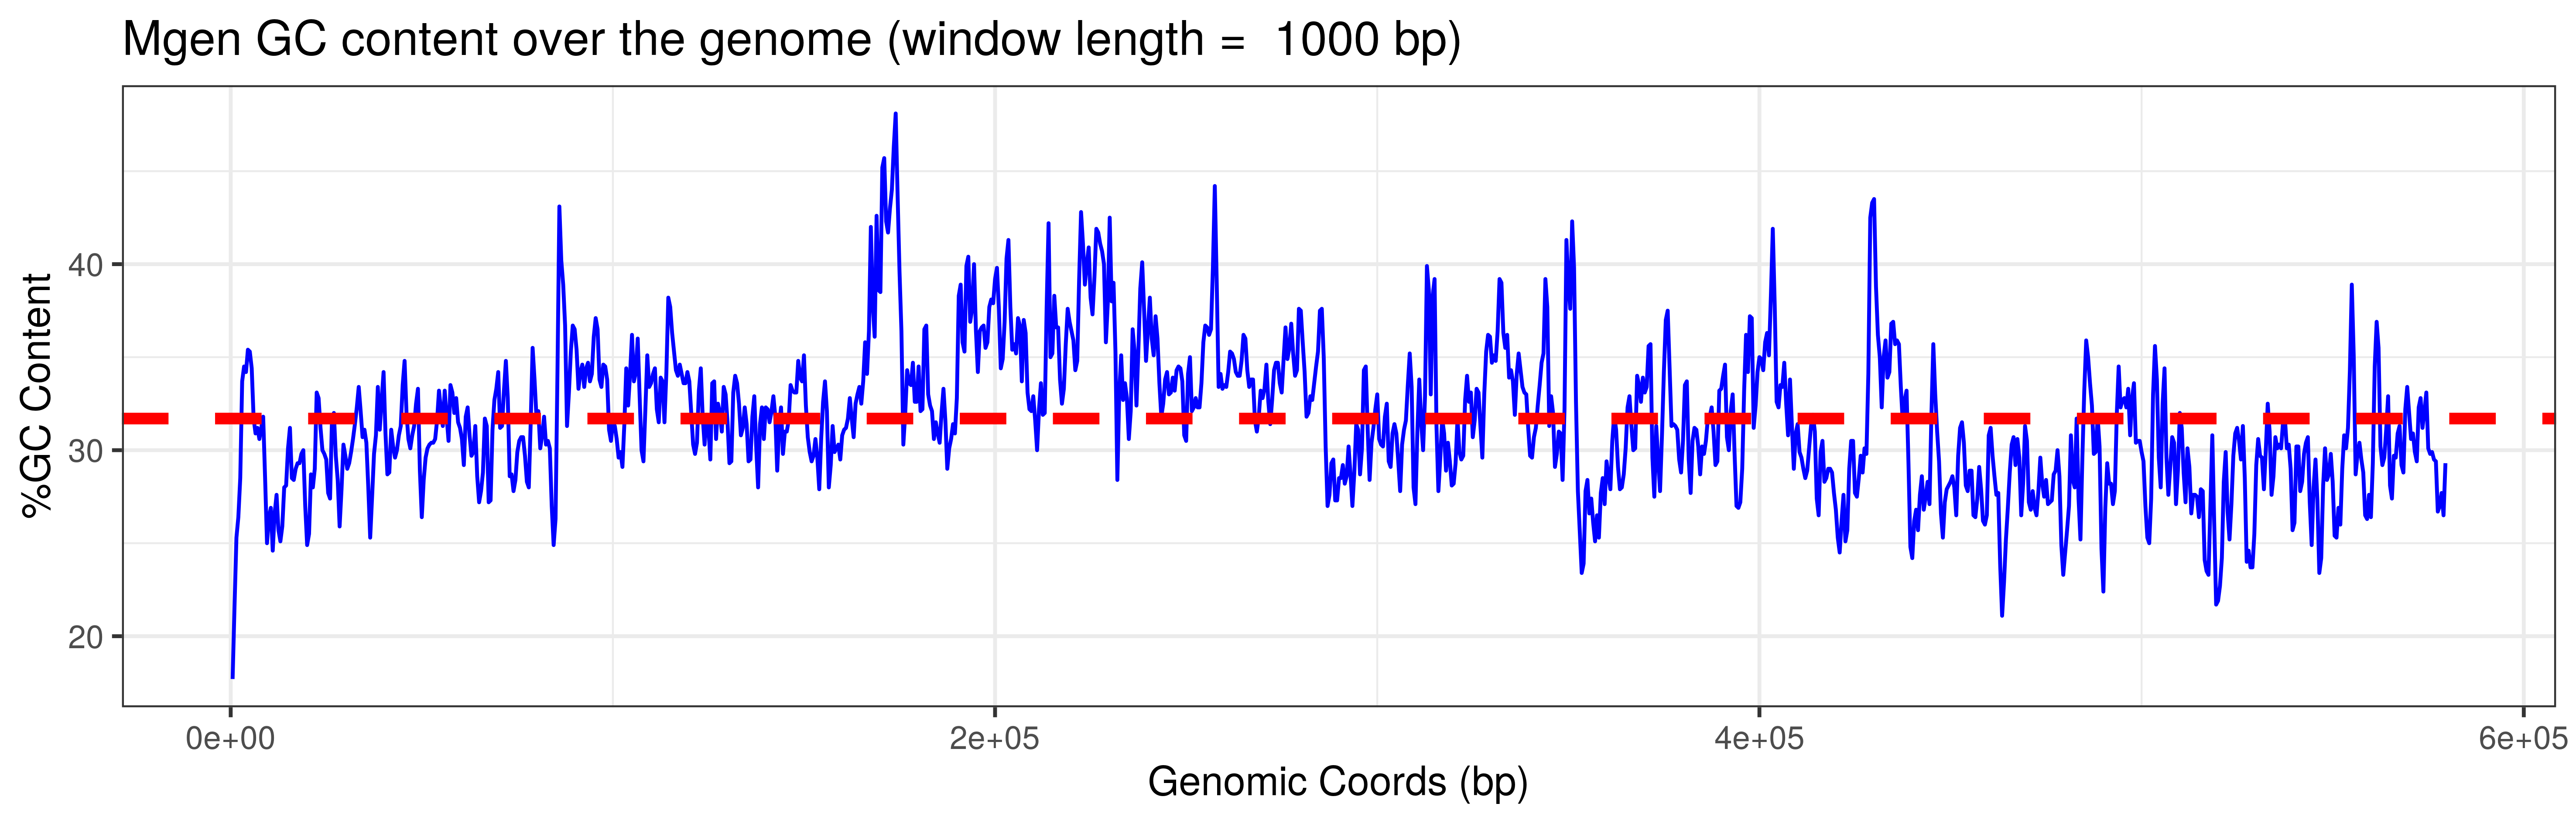
\includegraphics[width=0.5\linewidth]{{images/Mgen_genomegcanalysis_wlen1000}.png}\\
 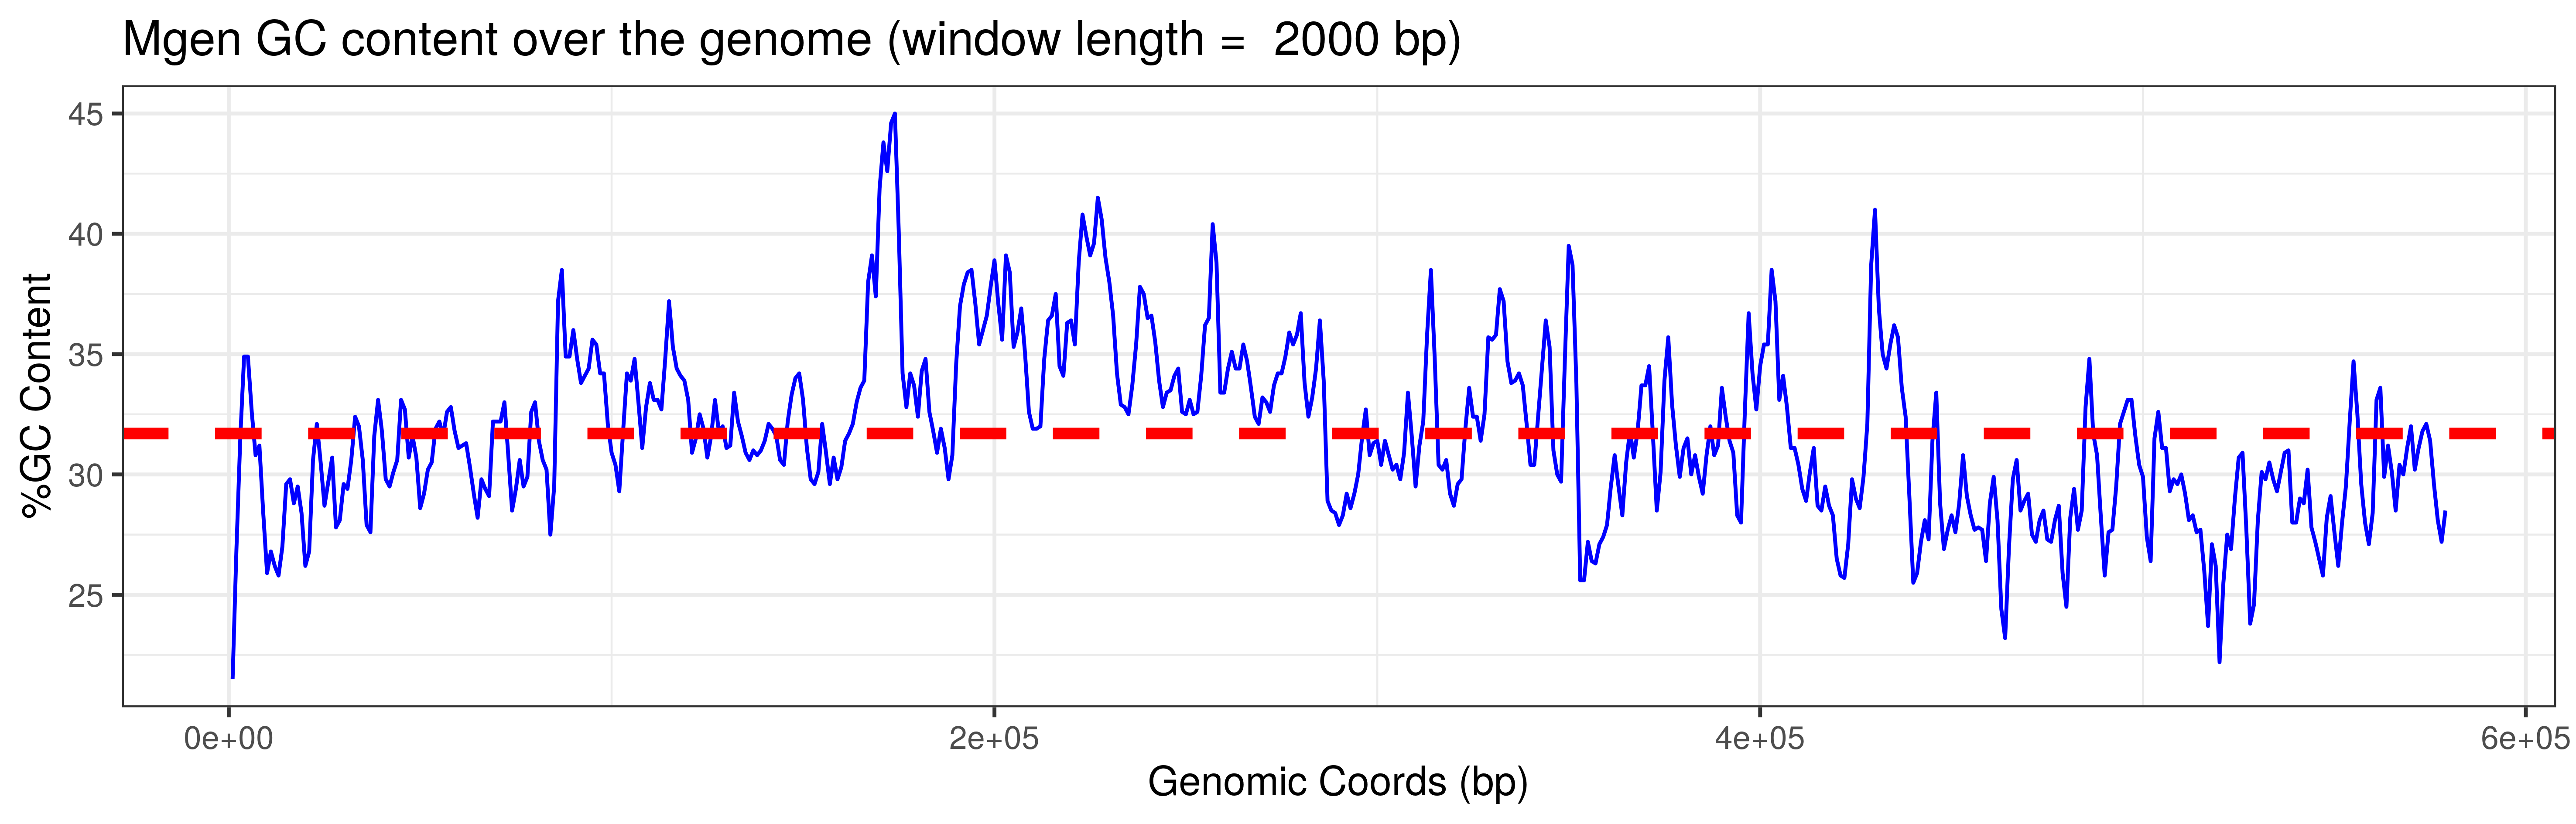
\includegraphics[width=0.5\linewidth]{{images/Mgen_genomegcanalysis_wlen2000}.png}\\
 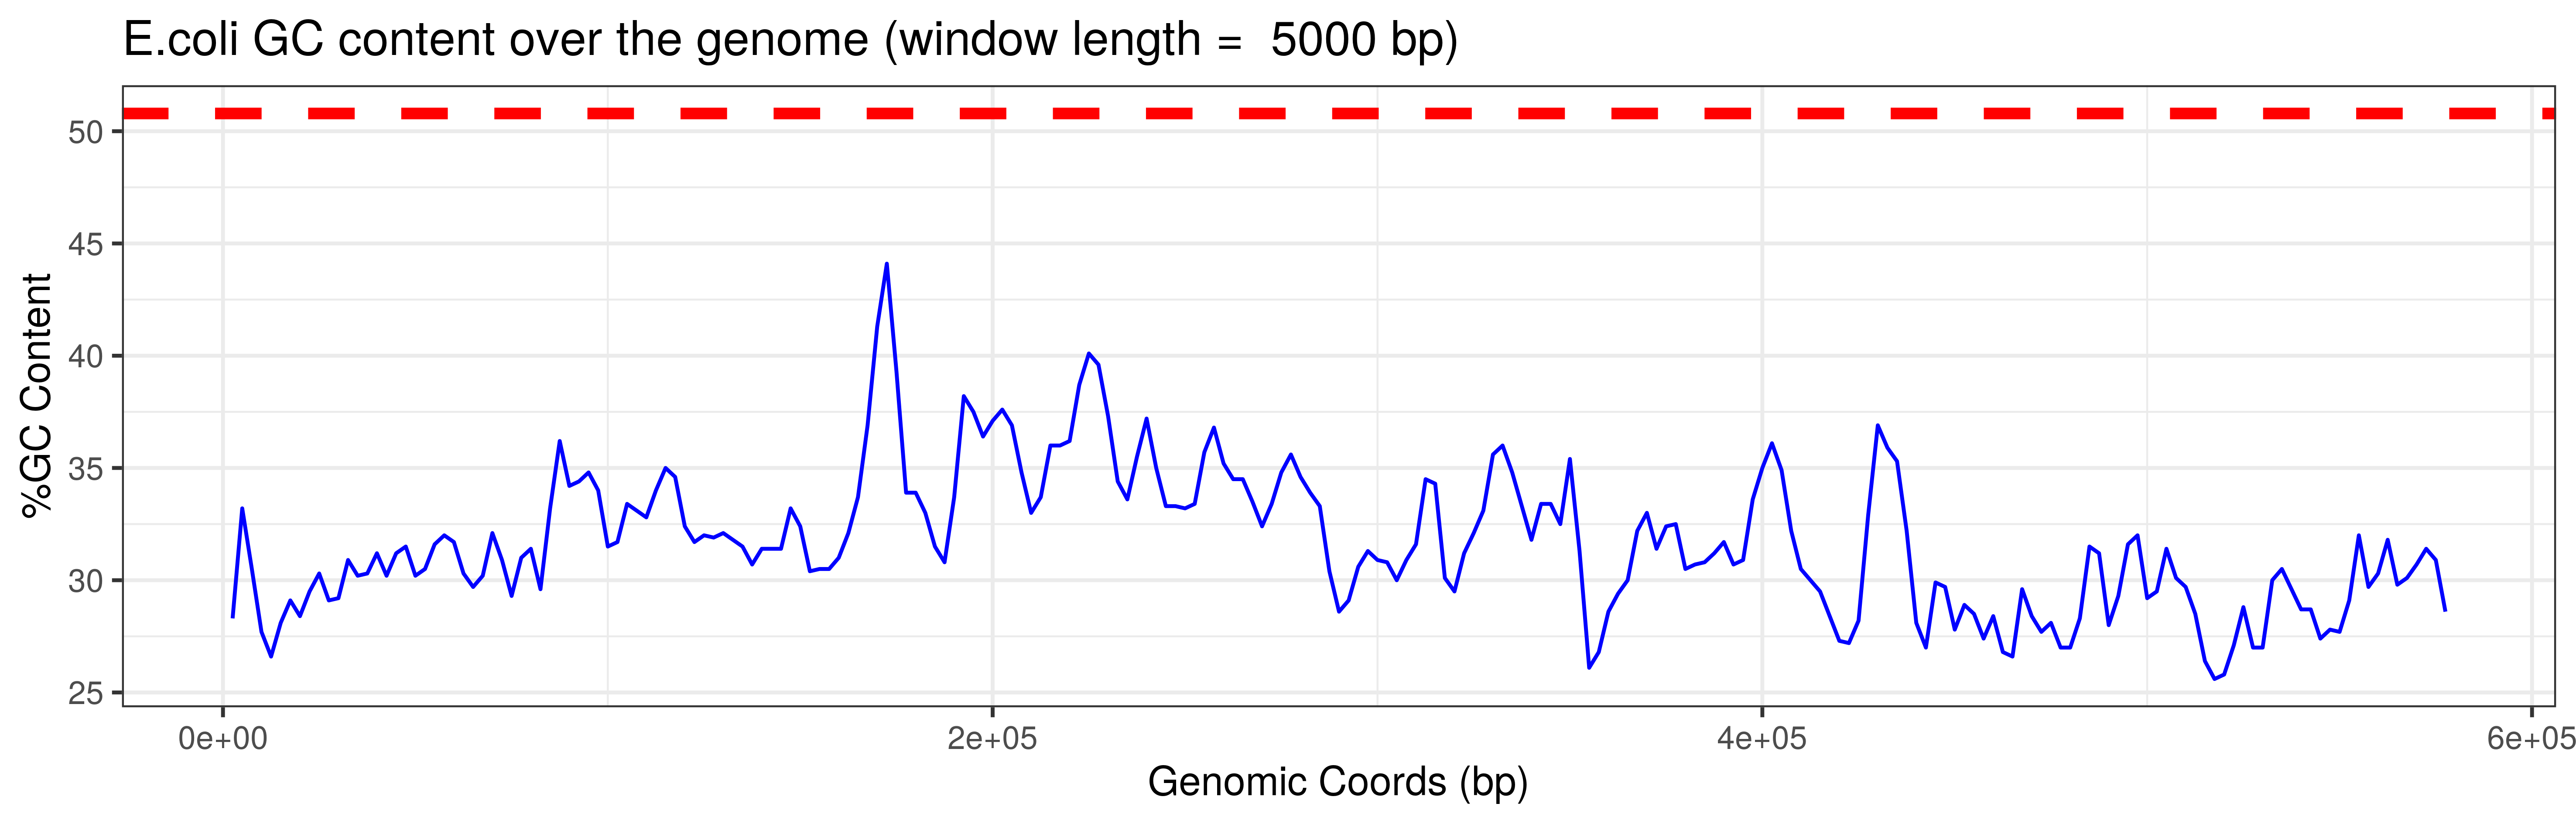
\includegraphics[width=0.5\linewidth]{{images/Mgen_genomegcanalysis_wlen5000}.png}\\
 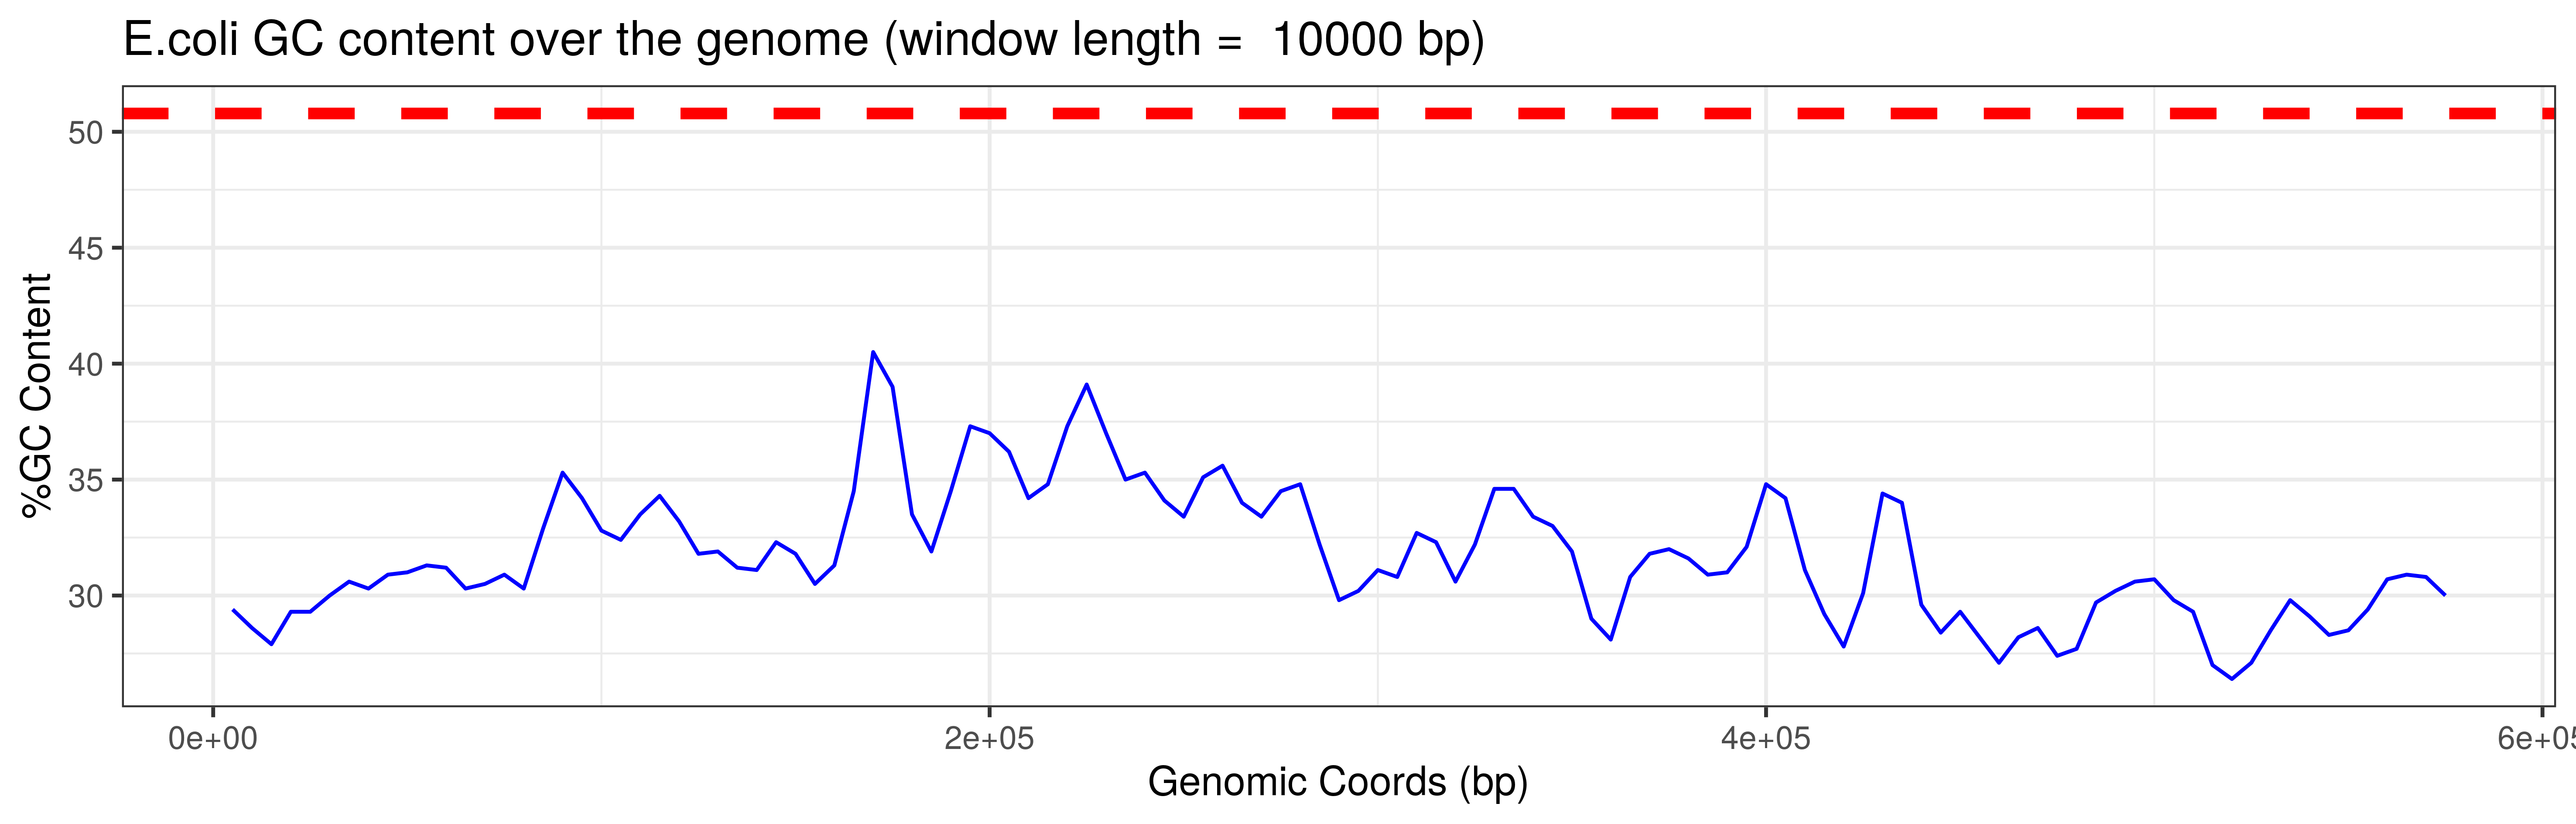
\includegraphics[width=0.5\linewidth]{{images/Mgen_genomegcanalysis_wlen10000}.png}\\
\end{center}

\caption[\cele\ Windows analysis of M.gen. for different sizes.]{%
  \label{fig:winlength}\textbf{\cele\ Windows size analysis.}
}%
\end{figure}

%

\begin{figure}[!h]
  \centering
  \begin{subfigure}[A]{\textwidth}
    \centering
    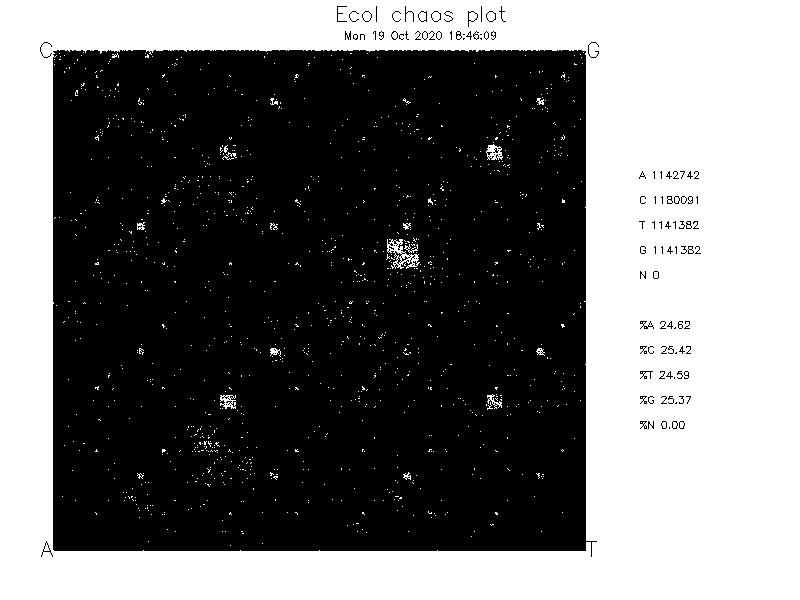
\includegraphics[width=0.4\textwidth]{{images/Ecol_chaosplot.1}.png}
  \end{subfigure}
  \hfill
  \begin{subfigure}[B]{\textwidth}
    \centering
    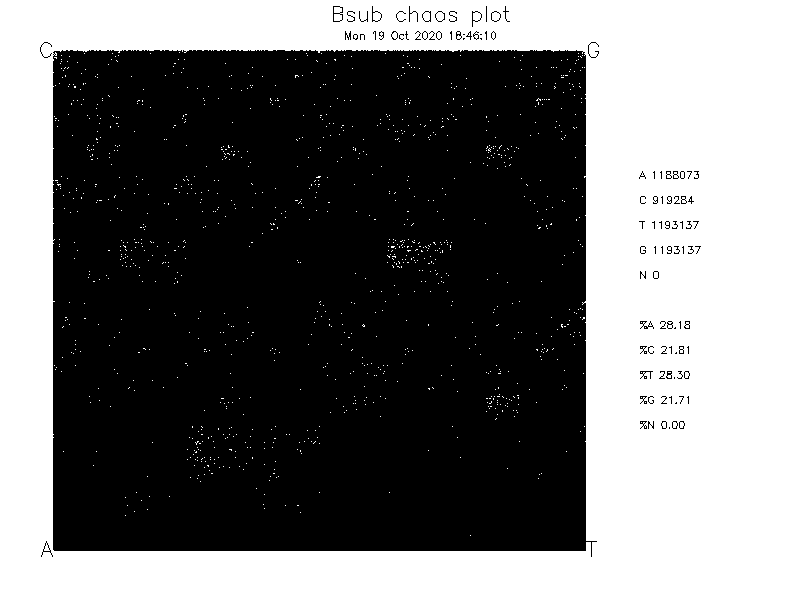
\includegraphics[width=0.4\linewidth]{{images/Bsub_chaosplot.1}.png}
  \end{subfigure}
  \vskip\baselineskip
  \begin{subfigure}[C]{\textwidth}
    \centering
    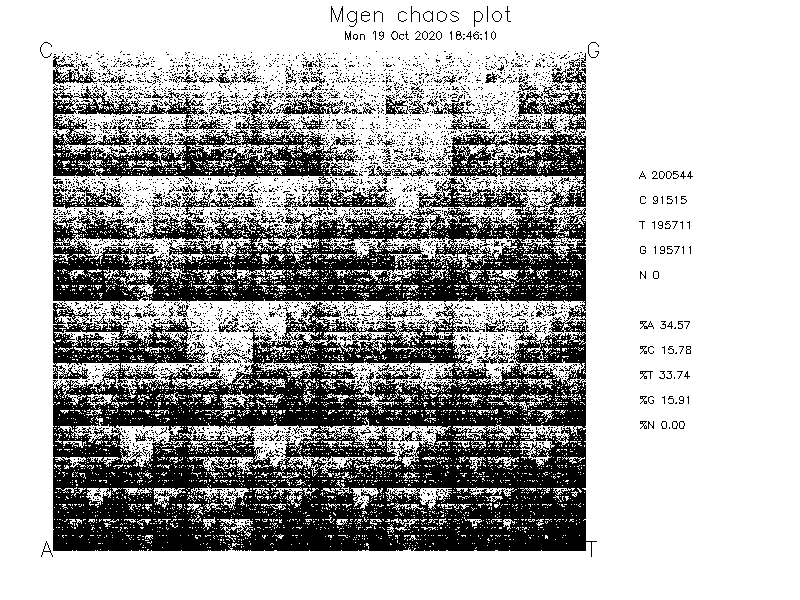
\includegraphics[width=0.4\linewidth]{{images/Mgen_chaosplot.1}.png}
  \end{subfigure}
  \hfill
  \begin{subfigure}[D]{\textwidth}
    \centering
    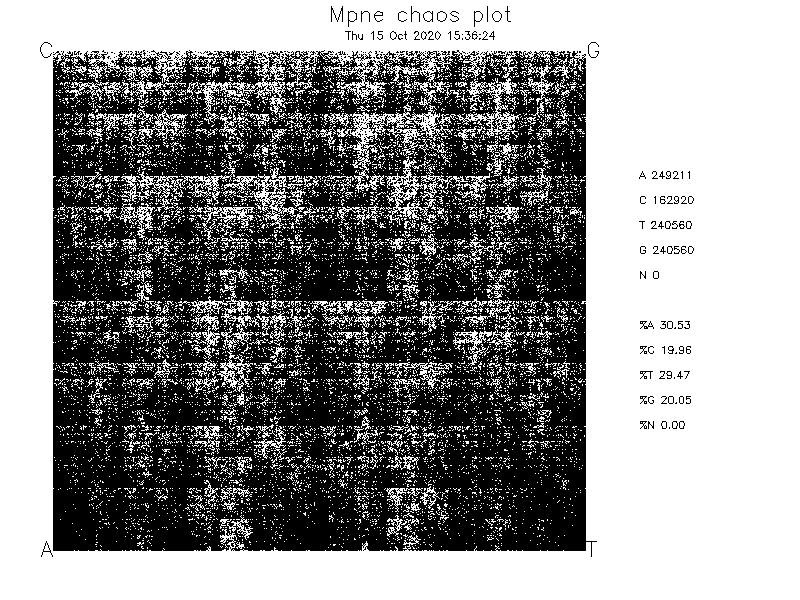
\includegraphics[width=0.4\linewidth]{{images/Mpne_chaosplot.1}.png}
  \end{subfigure}
\caption[\cele\ Chaos plot for different genomes species.]{%
  \label{fig:chaosplot}\textbf{\cele\ Chaos plot.}
}%
\end{figure}
